\newtheorem{definition}{\textbf{Definice}}

\chapter{Úvod}
\label{ch:uvod}

V dnešní době, je obor umělé inteligence(AI), postupem let všudypřítomnější a její vliv ovlivňuje sloustu aspektů našeho života.

Pokrok umělé inteligence je často a nejlépe měřen její aplikováním v oblasti her.
A to proto, že právě hry nabízí jasně definovaná pravidla a cíle, čímž se stávají ideálním testovacím prostorem pro algoritmy umělé inteligence.
Výkon AI je ve hrách snadno měřitelný a pokrok dokáže vidět i lajk bez žádných složitých grafů a výpočtů.
Umělá inteligence již dokázala porazit nejlepší hráče v \textit{šachu}~\cite{DeepBlue}, \textit{Dota 2}~\cite{Dota2}, \textit{Go}~\cite{AlphaGo} a spoustě dalších her.

Hra studovaná v této práci se jmenuje \emph{Scotland Yard}.
Jedná se o hru pro tři až šest hráčů.
V této hře obvykle hraje jeden hráč jako Pan X, který se snaží uniknout policistům, ovládanými ostatními hráči.
Policisté, avšak nevědí, kde na herním poli se Pan X nachází.
A musí tedy odhadovat jeho pozici a spolupracovat mezi sebou, aby ho mohli polapit.
Pozice Pana X je policistům odhalena pouze v určitých kolech.
Hra je u konce, když Pan X chycen policisty (vyhrávají policisté), nebo když je dosažen maximální počet kol (vyhrává Pan X).
Scotland Yard je ideální hrou ke studování neučitosti ve hrách hranýmy systémy umělé inteligence, protože se jedná o hru s nedokonalou informací a k vítězství policistů je zapotřebí spolupráce a strategie.

Tato práce zkoumá algoritmy posilovaného učení, jejich použití na hry s neurčitostí a jejich porovnání s klasickými metodami hraní her.
Algoritmus proximální optimalizace politiky (Proximal Policy Optimization--PPO) je hlavním zkoumaným algoritmem této práce.
Pro srovnání s jinýmy algoritmy slouží algoritmus Deep--Q--Learning (DQN).
PPO je často používán k řešení problémů se spojitými veličinami a ve 3D prostoru.
Algoritmus PPO byl vybrán z důvodu jeho úspěšnosti při použití ve složitých hrách s neurčitostí.
Tyto tvrzení podporuje experiment OpenAI~\cite{PPO_Hide_Seek_page}, podrobně popsán zde\cite{PPO_Hide_Seek_paper}.
V tomto experimentu byla proximální optimalizace politiky použita pro učení politiky ve hře typu \textit{schováváná} s několika agenty a neúplnou informací.
Jelikož tento typ hry přesně odpovídá i hře Scotland Yard, zdá se být vhodný i pro řešení této hry.
Také další studie~\cite{Manille} a \cite{Dota2} tento výrok dále podporují a dokazují vhodnost algoritmu PPO pro tuto práci.

Zaměření této práce jsem si vybral, jelikož mi vždy byla umělá inteligence blízká a vždy jsem chtěl začít tomuto odvětví více věnovat i po praktické stránce.
Algoritmus je pro mě zajímavý a zkušenost s tímto algoritmém by se dala využít v mém dalším pracovním životě.\newpage

Pro zpracování práce byly využity tyto hlavní knihovny:
\begin{itemize}
  \item \emph{Ray.Rlib} - framework pro posilované učení. Obsahuje již zhotovenou implementací algoritmu PPO a DQN, které byly použity v této práci. 
  \item \emph{PyTorch} - podpůrná knihovna Ray.Rlib
  \item \emph{Gymnasium} - knihovna použita k vytvoření prostředí hry Scotland Yard
  \item \emph{Pygame} - knihovna pro vytváření uživatelského rozhraní
\end{itemize}

Práce byla zhotovena pro operační systémy Windows a Python verze 3.10

\chapter{Shrnutí dosavadního stavu}
\label{ch:dosavadni_stav}
Tato kapitola není encyklopedickým přehledem celého tématu bakalářské práce.
Nýbrž jedná se o shrnutí nejdůležitějších relevantních informací a pojmů, důležitých pro tuto práci.

\section{Desková hra Scotland Yard}
\label{sec:deskova-hra-scotland-yard}

Scotland Yard je populární hra pro tři a více hráčů, která kombinuje prvky schovávané a hry na honěnou.
Jeden hráč hraje za Pana X, který se snaží uniknout policistům a ty ovládají zbylí hráči.
Hra končí, když je Pan X chycen (vyhrávají policisté), nebo když je dosažen maximální počet kol (vyhrává Pan X).
Originální hra se odehrává v na mapě Londýna.

\begin{figure}[H]
	\centering
	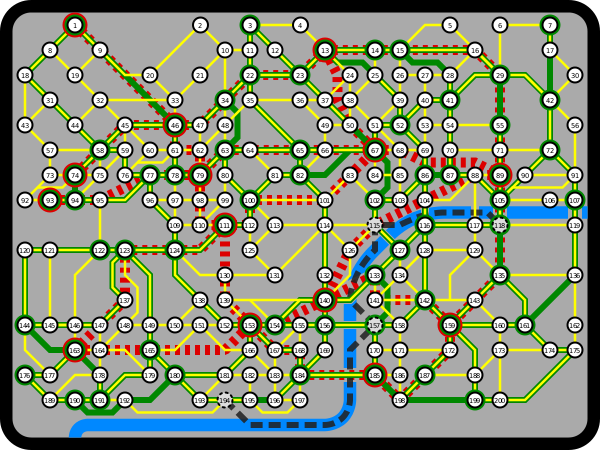
\includegraphics[width=0.9\textwidth]{obrazky-figures/scotland_original}
	\caption{Ukázka herní mapy hry Scotland Yard.
  Zdroj: \cite{scotland_original_image}}\label{fig:figure}
\end{figure}
\newpage

Na této herní mapě nachází 200 polí, které jsou vzájemně propojené náhodnými cestami.
Každá z těchto cest povoluje pouze určitý způsob dopravy (např. pouze taxíkem, pouze autobusem atd.).
Jednotliví hráči využívají prvky veřejné dopravy k pohybu po herní ploše, kterými jsou:

\begin{itemize}
  \item \emph{Taxi}\vspace{-0.3cm}
  \item \emph{Autobus}\vspace{-0.3cm}
  \item \emph{Metro}\vspace{-0.3cm}
  \item \emph{Trajekt}\vspace{-0.3cm}
\end{itemize}


Každému hráči je na začátku hry přidělen pouze určitý počet jízdenek na tyto dopravní prostředky.
K využití dopravy je potřebná právě tato jízdenka.
Pokud jízdenku hráč nemá, nemůže již tento způsob přepravy použít.
Hra se dělí na kola, ve kterých se hráči střídají.

Hlavní zápletkou hry je, že po většinu kol je pozice Pana X policistům utajena.
Odhaluje se jim pouze určená kola.
To znamená, že policisté pro polapení Pana X musí odhadovat jeho pozici a spolupracovat mezi sebou.
Tímto se ze hry Scotland Yard stává hra s nedokonalou informací, jelikož policisté nevidí přesnou pozici Pana X\@.
Tento fakt ji činí vhodnou pro studování metod hraní her s neurčitostí.

\section{Další hry s nedokonalou informací}\label{sec:dalsi-hry-s-nedokonalou-informaci}
V oblasti umělé inteligence hraje důležitou roli modelování a řešení her.
Hry představují formalizaci konfliktních interakcí mezi aktéry.
Klasická teorie her se zaměřuje na hry s úplnou informací, kde mají všechny strany v daném okamžiku přístup ke všem relevantním informacím z herního prostředí.
Znají strategie a cíle ostatních hráčů.
V praxi se však častěji setkáváme se situacemi, kde jednotlivým stranám chybí některé informace, ať už se jedná o prostředí či cíli soupeře.

\subsection{Bayesovské hry}
Tyto případy lze modelovat pomocí her s neúplnou či nedokonalou informací, kde hráči nemají úplné znalosti o prostředí nebo soupeřích.
Neúplnou informaci můžeme sledovat například u Bayesovských her.

\begin{definition}[Bayesovská hra]
\cite{Y_Narahari} je definována pěticí $(N, A_i, \theta_i, p(\theta_i), u_i)$, kde:

\begin{itemize}
\item $N$ je konečná množina hráčů, $N = \{1, 2, \ldots, n\}$.
\item $A_i$ je neprázdná množina strategií hráče $i$.
\item $\theta_i$ je neprázdná množina typů hráče $i$.
\item $p(\theta_i)$ je apriorní pravděpodobnostní rozdělení typu hráče $i$ na $\theta_i$.
\item $u_i: A_1 \times \cdots \times A_n \times \theta_1 \times \cdots \times \theta_n \rightarrow \mathbb{R}$ je výplatní funkce hráče $i$.
\end{itemize}
\end{definition}

Bayesovské hry představují formální rámec sloužící k modelování a popisu her s neúplnou informací.

\subsection{Stratego}\label{subsec:stratego}
Stratego je desková strategická hra pro dva hráče
Vychází z dřívějších her, jako je Šachy a Go, a kombinuje strategické plánování se snahou obelstít soupeře.
Hra se odehrává na herní ploše o velikosti 10x10 polí.
Na této herní mapě má každý hráč svoji sadu figur reprezentujících armádu.
Figury jsou ale vyobrazeny tak, že jejich hodnost lze přečíst pouze z jedné strany.
Tím druhý hráč nezná, rozestavění protivníkovy armády.

Každý hráč má 40 figur, rozdělených do 11 hodností (generál, plukovník, skaut atd.).
Cílem hry je porazit soupeře nalezením a obsazením jeho vlajky.
S vlajkou, stejně tak s minou nemohou hráči po umístnění pohnout.
Tyto speciální miny mohou zničit jakoukoliv figuru se kterou se utkají v boji.
Minu může zničit pouze horník.

Hra začíná tím, že každý hráč rozmístí své figury na herní pole.
Hráči se střídají v tazích, kdy se pokouší najít oponentovu vlajku.
Pokud hráč táhne na pole, kde se nachází oponentova figura, nastává souboj.
Souboj spočívá v odkrytí hodnosti obou figur a vyhrává ta s vyšší hodností.
Figura, která vyhrála zůstává, poražená figura je odstraněna z hry.

Ve hře Stratego je důležité blafování a odhadování soupeřových tahů.
V této hře velmi důležitá informace, tudíž je důležité informace získávat.
To můžou hráči učinit například obětováním slabších figur, aby odhalily silnější hodnosti.

\begin{figure}[H]
	\centering
	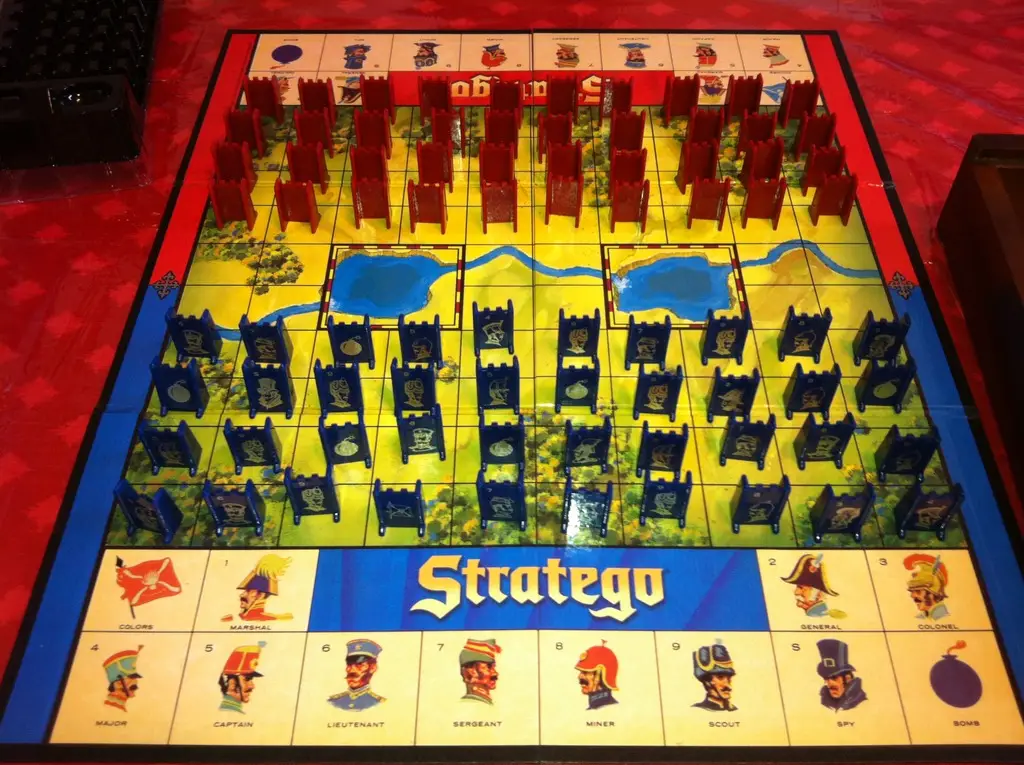
\includegraphics[width=0.6\textwidth]{obrazky-figures/stratego}
	\caption{Ukázka rozestavěných figur ve hře Stratego.
  Zdroj: \cite{Stratego_image}}\label{fig:figure2}
\end{figure}

Z pohledu umělé inteligence je Stratego zajímavý problém.
Nejenže je hra s nedokonalou informací a je tedy zapotřebí odhadovat oponentovy tahy a blafovat.
Hra ale také má obrovský stavový prostor $10^{535}$\cite{Perolat_2022}, čímž je prakticky neřešitelná klasickými metodami, které prochází celý stavový prostor.
Až do roku 2022 nebyla umělá inteligence v této hře velmi úspěšná a nedokázala se rovnat expertním hráčům.
To se změnilo příchodem \emph{DeepNash}\cite{Perolat_2022}, kdy se tento agent umístil mezi třemi nejlepšími hráči světa.

\subsection{Dota 2}\label{subsec:dota}
Dota 2 je velmi komplexní strategická hra v odehrávající se v reálném čase.
Hraje se ve dvou týmech po pěti hráčích.
Každý tým má svoji základnu, kterou se snaží chránit a zároveň zničit základnu soupeře.
Hra je u konce v okamžiku, kdy je zničena základna jednoho z týmů a tento tým prohrává.
Herní mapa se skládá ze tří hlavních cest, které jsou spolu navzájem propojeny mnoha menšími stezkami.

V každém týmu hraje 5 hráčů, kteří ovládají postavy s různými unikátními schopnostmi.
Hráči získávají zkušenosti jak za porážení nepřátelských postav, tak za zabití jednotek ovládaných počítačem.
Zkušenosti se využívají k zvyšování úrovně postavy a odemykání nových schopností.
Schopnosti jsou hlavní součástí hry.
Díky schopnostem mohou hrdinové zranit nepřítele, udělat silnější sebe či své spojence a mohou mít i spousty dalších efektů.
Co jim navíc přidává na komplexnosti je to, že každá schopnost nemůže být po použití znovu použita po určitou dobu.
Zlato používají hráči jako herní měnu, za kterou si hrdinové mohou koupit různé předměty, které je posílí.

Ve hře se vyskytuje válečná mlha, která způsobuje že hráči vidí pouze část mapy ve svém okolí a okolí spřátelených jednotek.
To znamená, že hráči nemají úplnou informaci o pozici nepřátelských jednotek.

\bigskip

Dota 2 je pro umělou inteligenci náročnou výzvou z těchto důvodů:
\begin{itemize}
  \item Složitost hry
  Dota 2 je komplexní hra s mnoha proměnnými a možnostmi.
  Její stav se mění velmi rychle a je tedy těžké předpovědět vývoj hry.
  Agenti tedy musí být schopni rychle reagovat na změny a tím přizpůsobit svoji strategii.
  \item Nedokonalá informace
  Právě kvůli válečné mlze nemají hráči úplnou informaci o pozici nepřátelských jednotek a musí tedy pouze odhadovat kde na mapě se nachází.
  Neznají ani jestli jsou nepřátelé schopni použít své schopnosti a předměty.
\end{itemize}

Dota 2 sama o sobě obsahuje implementaci chování umělé inteligence.
Její výkon však není dostatečný a nebyla schopna ani zdaleka porazit nejlepší hráče světa.
Použité metody pro vytvoření těchto agentů bohužel nejsou zveřejněny.

\ref{subsec:dota}
Inovaci umělé inteligence v této hře opět přinesla společnost OpenAI a jejich projekt \emph{OpenAI Five}\cite{Dota2}.
Tento projekt se zaměřil na vytvoření agenta, který by byl schopna porazit nejlepší hráče světa ve hře Dota 2.
OpenAi nepřišel se žádným novým algoritmem, ale pouze s novým přístupem k trénování a využití algoritmu \textbf{PPO} v doposud neviděném měřítku. 
Algoritmus PPO a posilované učení bodou blíže popsáni v následujících sekcích \ref{sec:proximalni-optimalizace-politiky} a \ref{sec:klicove-koncepty-posilovaneho-uceni}.

OpenAi Five porazil tehdejší nejlepší tým světa během exibice na nejprestižnejším turnaji Dota2 \textit{The International}.
Hrála se klasická turnajová verze, a to tedy nejlepší ze tří.
OpenAI Five byl schopen porazit nejlepší tým světa s rozhodným výsledkem 2:0.
První hra trvala 38~minut a druhá již pouhých 21~minut.
V celém exhibičním turnaji proti nejlepším týmům světa z celkových 24 her vyhrál 19 her a pouhých 5 prohrál.

Agent OpenAI Five byl, kombinovaně s předchozí verzí, trénován asi \emph{55 000} herních let hraním sama proti sobě.
Pozorovací prostor je obrovský, obsahuje až 16 000 vstupů.
Akční prostor je složitý, jelikož lidé hrají Dotu 2 většinou pomocí myši a klávesnice.
U OpenAI Five je akční prostor rozdělen na hlavní akce a parametry těchto akcí.
Hlavní akce jsou například, pohyb, útok, použití schopnosti/ předmětu, zakoupení předmětu a další situační akce.
Dostupnost těchto akcí je závislá na stavu hry a je řízena maskou akcí.
Tyto akce mají 3 parametry, zpoždění, vybranou jednotku a offset cíle akce.
Pokud tyto akce a jejich parametry zkombinujeme získáme akční prostor o velikosti 1,837,080 dimenzí.
Výsledný reakční čas agenta je okolo 33ms, oproti tomu reakční čas profesionálních hráčů her je okolo 120ms\cite{reaction_time}

Na začátku byla většina chování agenta uměle naprogramované a postupně mu byla předávána kontrola nad vlastním chováním s využití politiky.
Některé skriptované chování však bylo zachováno i ve finální verzi OpenAi Five a nebyly odstraněny, jelikož již agent byl dostatečně efektivní a nebylo třeba je odstranit.

\section{Klíčové koncepty posilovaného učení}\label{sec:klicove-koncepty-posilovaneho-uceni}
Posilované učení (Reinforcement Learning, RL) je oblast strojového učení, která se zaměřuje na učení agentů v dynamickém prostředí.
Agent se učí strategii chování, která maximalizuje kumulativní odměnu.

\subsection{Agent}\label{subsec:agent}

Je komplexní entita, která interaguje s prostředím.
Prostředí poskytuje agentovi informace o stavu a agent na základě těchto pozorování vykonává akce.
Tyto akce mohou ovlivnit stav prostředí a agent obdrží odměnu na základě odměnové funkce.
Agent většinou volí takové akce, aby maximalizoval kumulativní odměnu.

\subsection{Pozorovací a akční prostor}
\label{subsec:prostory}

\textbf{Pozorovací prostor} je jednou z nejdůležitějších součástí posilovaného učení.
Bez jeho vhodného zvolení, je dosažení politiky s dobrými výsledky velmi obtížné.
Pozorovací prostor je množina všech možných pozorování, které může agent získat z prostředí.
Je to tedy forma, kterou prostředí předává informace agentovi.
Velmi často se aktuální stav pozorovacího prostoru využívá jako stav.
Při vytváření prostředí je nutné definovat typ, tvar prostoru a jaké hodnoty může nabývat.

Pro jeho podoby je vhodné zvolit standard z knihovny \emph{Gymnasium}\cite{Gymnasium}.
Gymnasium je pokračování knihovny \textit{Gym} od společnosti OpenAI.
Tyto knihovny nastavily standard vytváření prostředí pro posilované učení.
Dodržování těchto standardů umožňuje použití libovolného algoritmu na jedno prostředí.

\bigskip

\textbf{Akční prostor} je, jak název vypovídá, množina všech možných akcí, ze kterých může politika volit.
Často se jedná o množinu celočíselných hodnot, které reprezentují různé akce.
Samozřejmě může být akční prostor i spojitého typu (blíže popsáno v další sekci).

V herním prostředí mohou nastat situace kdy se nějaká akce stane nevalidní, jelikož by její provedení vyústilo v nevalidní stav herního prostředí.
V takovém případě je vhodné zvolení této akce zamezit, nejlépe pomocí akční masky.
Ta definuje, které akce jsou v momentálním stavu prostředí proveditelné.

\subsection{Diskrétní a spojitý prostor}\label{subsec:diskretni-a-spojity-prostor}

Pokud se bavíme o \textbf{diskrétním prostoru} v oboru umělé inteligence, bavíme se o konečném prostoru prostoru. 
Skládá se tedy z konečného počtu prvků.
Příkladem takového prostoru je například pozorovací prostor, jehož vstupem je fotka.
Ta se dělí na přesně daný pošet pixelů a je tedy diskrétní.
Dískrétní akční prostory jsou počítatelné a často se jedná o konečnou množinu možných akcí.

Zato \textbf{spojitý prostor} je nekonečný prostor, který může obsahovat nekonečný počet prvků. 
Spojitý pozorovací prostor je například ten, jehož vstupem je audio stopa.
Spojité akční prostory jsou nekonečné a často je definuje nekonečná množina akcí.
Na prostředí se spojitýmy prostory se často používají jiné algoritmy, například algoritmus DDPG (Hluboký deterministický gradient politiky).

\bigskip

Uvažujme však 3D hru kde se agent může hýbat za pomocí aplikování silového vektoru o různé velikosti a v různém směru.
Může tím tedy měnit rychlost a směr pohybu.
V tomto případě se jedná o \textbf{spojitý akční prostor}.

\subsection{Prostředí}\label{subsec:prostredi2}

Je vše s čím agent interaguje.
Prostředí je buď fyzické (entity z reálného světa, ovládání chytré domácnosti, robotické ruky, ovládání reaktoru apod.) nebo virtuální (simulace nebo hra).
Prostředí reaguje na zvolené akce agenta poskytuje mu zpětnou vazbu ve formě odměny.
Odměna může být i záporná, pokud agent zvolil velmi nevhodnou akci.
Pokud v prostředí existuje více agentů, může mít každý agent jiné pozorování.
Díky tomuto můžeme například schovat agentovi \textit{A} určité informace, které agent \textit{B} vidí.

\subsection{Politika}\label{subsec:politika}

Pomocí posilovaného učení vzniká takzvaná politika.
V češtině se také může pojem politika přeložit jako strategie.
Politika je matematická funkce, která definuje agentovo chování na základě jeho pozorování (stavu).
Snaží se definovat takové chování, které vede k maximální kumulativní odměně.
Politika může být deterministická nebo stochastická.

  \subsubsection*{Deterministická politika}
  
  Deterministická politika přesně definuje cílový stav přechodu pro každý stav.
  Agent tedy pro jeden stav vždy volí stejnou akci.
  Tato politika je vhodná, pokud je zapotřebí v každém stavu reagovat konzistentně, bez odchylek.
  Například, pokud agent ovládá termostat v domě a teplota je pod požadovanou hladinu.
  Nemůže se stát, aby byla šance, že agent zvolí akci, která teplotu ještě sníží.
  Další výhoda, je že je jednoduchá na interpretaci a implementaci.\cite{Policies}

  Rovnice výsledné akce deterministické politiky je:
  \begin{equation}
    \pi(s) = a\label{eq:policy_deterministic}
  \end{equation}

  \subsubsection*{Stochastická politika}
  
  Zato stochastická politika definuje pro každý stav pravděpodobnostní rozdělení nad množinou akcí.
  Výsledná akce je tedy náhodná dle rozdělení pravděpodobnosti.
  Může tedy nastat situace kdy ve stejném stavu agent zvolí vždy jinou akci.
  Tato politika je vhodná v situacích, kdy je potřeba zkoumat různé strategie a kdy agent nemá úplnou informaci o prostředí.
  Například tam kde by deterministická politika zvolila jasnou akci \textit{A}, stochastická politika by mohla s malou pravděpodobností zvolit akci \textit{B}.
  Čímž ale může odhalit, že stav \textit{B} je s ohledem na komulativní odměnu lepší než stav \textit{A}.\cite{Policies}

  Rovnice výsledné akce stochastické politiky je:
  \begin{equation}
    \pi(a \vert s) = \mathbb{P}_\pi [A=a \vert S=s]\label{eq:policy_stochastic}
  \end{equation}

\subsection{Akce}\label{subsec:akce}

Akce je aktivita, proces či funkce kterou agent vykoná ve specifickém stavu \cite{ActionCo67}.
Výsledkem provedení akce je tedy změna z aktuálního stavu, do jiného, či stejného stavu z množiny možných stavů.
Zjednodušeně, je to rozhodnutí, které agent vykonává v prostředí a toto rozhodnutí ovlivňuje prostředí.

Akce může být také nedeterministická či stochastická.
Výsledný stav tedy může být stejný pro stejný stav a akci.
  
\subsection{Odměna}\label{subsec:odmena}

  Odměna je hodnota, kterou agent obdrží od prostředí po vybrání akce.
  Může být kladná, záporná nebo nulová.
  Dle této zpětné vazby se agent učí, jak moc byla jeho zvolená akce v daném stavu vhodná.

\subsection{Hodnotová funkce}\label{subsec:hodnotova-funkce}

  Hodnotová funkce vyhodnocuje, jak dobrý je stav tím, že predikuje budoucí odměnu, pokud bude další tah začínat v tomto stavu.
  Čím vzdálenější odměna je od tohoto stavu, tím více je snížena.
  Protože, čím je odměna vzdálenější tím více je nejistá, že bude doopravdy získána.

  Existují dva typy hodnotových funkcí:

  \subsubsection*{Hodnotová funkce stavu $V(s)$}

  Hodnotová funkce stavu \emph{$V(s)$} vyhodnocuje očekávanou komulativní odměnu, jestliže se agent nachází v tomto stavu.
  Tato funkce je závislá na politice, kterou se agent řídí.
  Vyhodnocuje tedy jak příznivý je daný stav pro agenta.

  \subsubsection*{Hodnotová funkce akce $Q(s, a)$}
  \label{subsubsec:q_function}

  Hodnotová funkce akce \emph{$Q(s, a)$} vyhodnocuje očekávanou komulativní odměnu, pokud se agent nachází v tomto stavu a zvolí tuto akci.
  Tato funkce je opět závislá na politice, kterou se agent řídí.
  Vyhodnocuje tedy jak příznivé je zvolení dané akce v aktuálním stavu.

\subsection{Markovský rozhodovací proces}\label{subsec:markovsky-rozhodovaci-proces}

Téměř všechny problémy, řešené posilovaným učením, mohou být označeny jako Markovy rozhodovací procesy (Markov Decision Process).
Tato abstrakce je základním kamenem pro modelování algoritmů posilovaného učení.
Markovský rozhodovací proces značí, že následující stav není závislý na stavech minulých, nýbrž pouze na aktuálním stavu.

\begin{figure}[H]
	\centering
	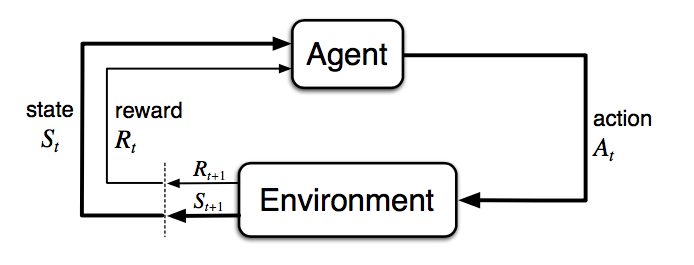
\includegraphics[width=0.6\textwidth]{obrazky-figures/RL_basics}
	\caption{Interakce mezi prostředím a agentem podle Markova rozhodovacího procesu.
  Zdroj: \cite{RL_basics}}\label{fig:markov}
\end{figure}

\begin{definition}
  
Markovský rozhodovací proces je definován pěticí $(S, A, P, R, \gamma)$\cite{RL_basics}, kde:

\begin{itemize}
\item $S$ je množina stavů.
\item $A$ je množina akcí.
\item $P$ je pravděpodobnostní přechodová funkce
\item $R$ je odměnová funkce
\item $\gamma$ je diskontní faktor pro budoucí odměny
\end{itemize}
\end{definition}

\subsection{Bellmanova rovnice}\label{subsec:bellmanova-rovnice}

Belmanova rovnice se zaměřuje na rozložení hodnotových funkcí na menší a snadněji zpracovatelné celky.
Dociluje toho tak, že rozděluje hodnotovou funkci na dvě části: \emph{okamžitou odměnu} a postupně snižovanou \emph{budoucí odměnu}.

\begin{equation}
  V(s) = E[R_{t+1} + \gamma V(S_{t+1}) | S_t = s]\label{eq:bellman1}
\end{equation}

\begin{equation}
  Q(s, a) = E[R_{t+1} + \gamma E_{a\sim\pi}Q(S_{t+1}, a) | S_t = s, A_t = a]\label{eq:bellman2}
\end{equation}



\subsection{Rovnováha mezi explorací a exploatací (exploration-exploitation dillemma)}
\label{subsec:exploration-exploitation-dillemma}
\begin{quote}
  \emph{Kompromis mezi potřebou získávat nové znalosti a potřebou použít již nabyté znalosti k vylepšení výkonnosti je jedním z nejzákladnějších kompromisů v přírodě.~\cite{Exploitation_Exploration}}
\end{quote}
Explorace a exploatace jsou dvě protichůdné strategie, které se vyskytují jak ve strojovém učení, tak i v reálném životě.

\emph{Exploatace} se snaží vybrat nejlepší možnou akci na bázi známých informací.
Tyto informace, nemusí být kompletní, nebo mohou být zavádějící.
A to z důvodu nedostatečného trénování, či nedostatečného prozkoumávání možností prostředí.

Tomu opačná metoda \emph{explorace} usiluje o prozkoumání možností, které nejsou známé a mohly by vést k lepší budoucí odměně.
Explorace tedy často zvolí akci, která nemusí být nejlepší, ale může odhalit nové informace, které následovně povedou ke zlepšení exploatace.

\subsection{Druhy informací v teorii her}\label{subsec:druhy-informaci-v-teorii-her}
V rámci umělé inteligence se potýkáme s různými druhy informací.
Dělí se na tyto hlavní typy:

\textbf{\emph{Dokonalá informace}} znamená, že agent ví o prostředí a o ostatních hráčích vše.
Například ve hře šachy.
Hráč vidí všechny figury na herní ploše, i ty soupeřovy.

\textbf{\emph{Kompletní informace}} značí, že agent je obeznámen se strukturou hry a jsou mu také odhaleny odměnové funkce ostatních hráčů.
Hráč tedy ví, jakou hru hraje je obeznámen s jejími pravidly.
A rozumí, jaké jsou podmínky výhry a je obeznámen s taktikou ostatních hráčů.

\textbf{\emph{Nedokonalá informace}} znamená, že agent nemá všechny relevantní informace o prostředí a ostatních hráčích.
Například, tedy všechny hry, ve kterých hrají hráči zároveň jsou hry s nedokonalou informací.
Jelikož hráč v daném okamžiku nezná informaci o tahu ostatních hráčů.
Další příklad je například hra poker, kde hráč nezná rozdané karty ostatních hráčů.
Také hra Scotland Yard, kde policisté neznají pozici Pana X\@.

\textbf{\emph{Neúplná informace}} znamená, že hráč nezná strukturu odměn, podstatu hry nebo její pravidla.
Hráč tedy nezná výchozí informace o hře.
Všechny hry s neúplnou informací se dají považovat za hry s nedokonalou informací.

\emph{Soukromá informace} je informace, která není dostupná ostatním hráčům.

\emph{Společná informace} je informace, která je dostupná všem hráčům.

Příklady
\begin{itemize}
  \item Nedokonalá ale kompletní informace - poker
    Karty ostatních hráču jsou skryté
    {\color {red} [DODĚLAT PŘÍKLADY]}


\end{itemize}


\section{Vhodné algoritmy k řešení her s nedokonalou informací}\label{sec:vhodne-algoritmy-k-reseni-her-s-nedokonalou-informaci}

Tato kapitola se zaměřuje na algoritmy, které jsou vhodné pro řešení her s nedokonalou informací, s důrazem na metody posilovaného učení a srovnáním s klasickými metodami jako Monte Carlo.

\subsection{Monte Carlo tree search}\label{subsec:monte-carlo-tree-search}
Metoda Monte Carlo tree search (MCTS) je heuristický algoritmus prohledávání.
Kombinuje stromové vyhledávání s principy posilovaného učení.
Je často využíván, je--li stavový prostor řešeného problém příliš velký a složitý na to, aby byl prohledán kompletně jinými metodami, jako například minimax, či alfa--beta prořezávání.
Tyto \uv{tradiční} algoritmy nelze na mnoho problémů použít, jelikož by byly příliš pomalé a náročné na výpočet.

Tato metoda se také potýká s rovnováhou mezi explorací a exploatací (viz.~ sekce~\nameref{subsec:exploration-exploitation-dillemma}).
Explorací se strom rozrůstá do šířky, zatímco exploatací se strom prohlubuje.

MCTS se skládá z několika fází:
\begin{itemize}
  \item \emph{Selekce}

  Na základě aktuálního stavu se vybere další stav k prozkoumání.
  Pro tento výběr se využívají dvě strategie:
  
  \emph{Strom s horní mezí spolehlivosti} (Upper confidence bounds applied to trees, UCT) kombinuje průměrnou hodnotu uzlu a odměnu za exploraci.

  \label{epsilon_greedy}
  \emph{Chamtivá strategie $\epsilon$ } ($\epsilon--greedy strategy$) vybírá s pravděpodobností $\epsilon$ náhodný uzel, jinak volí uzel s nejvyšší hodnotou.
  Tato strategie se používá méně často než UCT\@.

  Obě tyto strategie se snaží o rovnováhu mezi explorací a exploatací.
  \item \textbf{\emph{Expanze}}

  V tomto kroku se vyhledávací strom rozšíří o nový uzel, který je výstupem z předchozího kroku.

  \item \textbf{\emph{Simulace}}

  Po této fázi je provedena náhodná simulace od nového uzlu až do konečného stavu.

  \item \textbf{\emph{Aktualizace}}
  
  Díky nově nabitým informacím ze simulace, se zpětnou propagací aktualizují hodnoty uzlů ve stromě.

\end{itemize}

\begin{figure}[H]
	\centering
	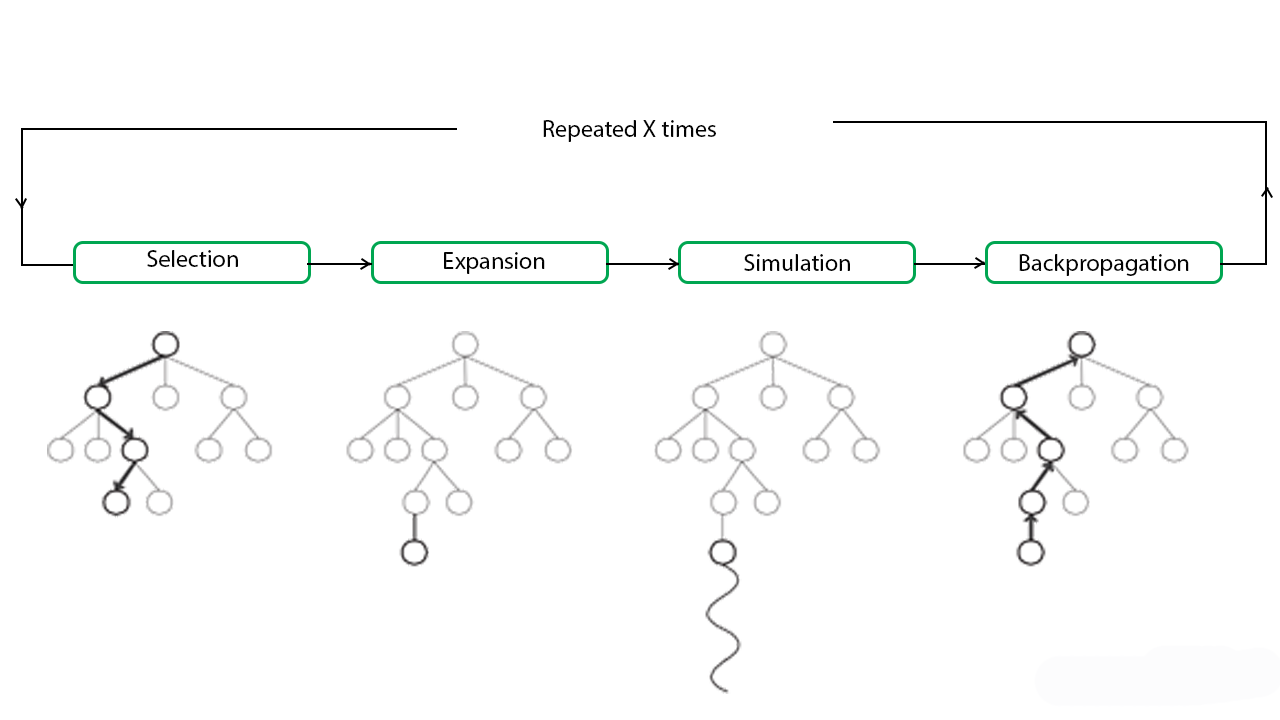
\includegraphics[width=0.9\textwidth]{obrazky-figures/mcts}
	\caption{Diagram jednotlivých fází MCTS.
  Zdroj: \cite{Monte_Carlo_Tree_Search}}\label{fig:mcts}
\end{figure}

Tento algoritmus se skvěle hodí na hry s nedokonalou či neúplnou informací, jelikož se spoléhá na vzorkování pomocí simulací.

\subsection{Q-learning}\label{subsec:q-learning}

Q-learning je jedním z nejznámějších algoritmů posilovaného učení.
Učení tohoto algoritmu probíhá bez modelu a mimo politiku.

Jak už název vypovídá, Q-learning se zaměřuje na určení hodnoty hodnotové funkci akce $Q(s, a)$, viz. \nameref{subsubsec:q_function}.
Tyto hodnoty se uchovávají v Q--tabulce, která na každou kombinaci stavu a akce uchovává hodnotu $Q(s, a)$.
Hodnoty v Q--tabulce se iterativně aktualizují na základě získaných odměn.
Kladná odměna po vykonání akce $s$, zvýší se hodnota $Q(s, a)$.
Naopak, dostane--li po vykonání této akce zápornou odměnu, hodnota $Q(s, a)$ se sníží.

Řádky Q-tabulky tedy reprezentují stavy a sloupce akce.
Po vytvoření jsou všechny $Q$ hodnoty v tabulce inicializovány na nulu.
Následně jsou tyto hodnoty iterativně aktualizovány dle zpětné vazby udělené od prostředí ve formě odměny.

Jako u většiny algoritmů je zde potřeba dohlédnout na rovnováhu mezi explorací a exploatací.
K tomuto se využívá $\epsilon$--greedy strategie viz. \nameref{epsilon_greedy}.

Hlavní nevýhodou tohoto algoritmu je právě jeho závislost na Q--tabulce.
Tabulka mapuje hodnoty pro každou kombinaci stavu a akce,
Je--li avšak stavový, či akční prostor příliš velký, nebo dokonce nekonečný je tento algoritmus nevhodný, skoro až nepoužitelný.
Výsledná Q--tabulka by byla neefektivní kvůli své velikosti.
Mohlo by se stát, že s nekonečným množstvím kombinací by velikost tabulky rostla do \uv{nekonečna}.
Jako řešení byl navrhnut algoritmus Deep Q-learning.

\subsection{Deep Q-learning (DQN)}\label{subsec:deep-q-learning}

Tato metoda je rozšířením algoritmu Q-learning které,
nahrazuje $Q$--tabulku neuronovou sítí určených k aproximaci hodnotové funkce akce $Q(s, a)$.
Díky této aproximaci je možné použít tento algoritmus na problémy s velkým, či nekonečným množstvím kombinací akcí a stavů.

Avšak tímto vzniká nový problém, \emph{nestabilita učení}.
Ten je řešen dvěma mechanizmy:

\begin{itemize}
  \item \textbf{\emph{Přehrání zkušenosti (experience replay)}}
  
  Během trénování se ukládají všechny zkušenosti do paměti.
  Ať už to jsou akce, stavy, odměny atd.
  Při trénování se poté náhodně vybírají náhodně zkušenosti z této paměti a aktualizují se podle nich váhy sítě.
  Tímto se snižuje rozdíl mezi jednotlivými aktualizacemi a tím pádem se zvyšuje stabilita učení.
  

  \item \textbf{\emph{Periodická aktualizace}}

  {\color{red}[DOPSAT!]}
  Síť je naklonována a změny se provádí pouze na duplikátní verzi.
  Do hlavní originální sítě se změny klonují po určitém počtu kroků.

\end{itemize}

Při vytváření neuronové sítě jsou váhy inicializovány náhodně.

\subsection{Gradient politiky}\label{subsec:gradient-politiky}
Oproti předchozím zmiňovaným algoritmům, které usilují o naučení hodnotové funkce či prohledávají stavový prostor, algoritmy gradientu politiky se snaží naučit politiku přímo.

V diskrétním prostoru je odměnová funkce definována jako:
\begin{equation}
  \label{eq:odmenova_funkce}
  \mathcal{J}(\theta) = V_{\pi_\theta}(S_1) = \mathbb{E}_{\pi_\theta}[V_1]
\end{equation}

V spojitém prostoru je odměnová funkce definována jako:
\begin{equation}
    \label{eq:odmenova_funkce_spojita}
  \mathcal{J}(\theta) = \sum_{s \in \mathcal{S}} d_{\pi_\theta}(s) V_{\pi_\theta}(s) = \sum_{s \in \mathcal{S}} \Big( d_{\pi_\theta}(s) \sum_{a \in \mathcal{A}} \pi(a \vert s, \theta) Q_\pi(s, a) \Big)
  \end{equation}

\subsubsection*{Věta o gradientu politiky}
Výpočet gradientu matematicky je zaznamenán touto rovnicí:

\begin{equation}
  \label{eq:gradient_politiky}
  \frac{\partial \mathcal{J}(\theta)}{\partial \theta_k} \approx \frac{\mathcal{J}(\theta + \epsilon u_k) - \mathcal{J}(\theta)}{\epsilon}
\end{equation}
Tento výpočet je velmi pomalý a náročný na výpočet.
Avšak tento vzorec lze zjednodušit na rovnici zvanou \emph{věta o gradientu politiky}:

\begin{equation}
    \label{eq:veta_o_gradientu_politiky}
  \nabla \mathcal{J}(\theta) = \mathbb{E}_{\pi_\theta} [\nabla \ln \pi(a \vert s, \theta) Q_\pi(s, a)]
\end{equation}

\section{Trust Region Policy Optimization (TRPO)}\label{sec:trust-region-policy-optimization}
Trénované politiky jsou často velmi náchylné na změny.
Kde i malá náhlá změna v jednom kroku může způsobit velké změny v chování agenta a zamezit dalšímu učení správné strategie.
Během učení totiž chceme, aby učení probýhalo plynule a ne skokově.
Pokud se politika změní příliš rychle protože následovala nějvětší růst, může se stát, že mine cestu vedoucí k optimální strategii.
Zasekne se tedy v lokálním optimu.

TRPO je optimalizační algoritmus, který se snaží tento problém řešit tím, že definuje omezení rozdílu mezi novou aktualizovanou politikou a starou politikou z předešlého kroku.
Tento rozdíl mezi dvěma pravděpodobnostními rozděleními je definován jako Kullback-Leiblerova divergence (K-L divergence)\cite{KL_divergence}.
Vzniká tak region důvěry, ve kterém musí nová politika setrvat.
Politika se tedy nemůže skokově měnit na lokální maximum, ale pouze následuje směr lokálního maxima.

K tomu využívá Hesenská matice.
Kdy pomocí těchto matic hledá optimální směr změny politiky.
Tím, že se hledá lokální maximum pouze v oblasti důvěry, řeší problém se zaseknutím v těchto lokálních optimech.

Díky tomuto řešení se učení stává robustním a stabilním.
Avšak výměnou za to, je náročnost aproximace pomocí Hesenských matic a s tím související náročnost na implementaci.

\section{Zkoumaný algoritmus proximální optimalizace politiky}
\label{sec:proximalni-optimalizace-politiky}

%\textsuperscript {\ref{sec:trust-region-policy-optimization}}

Metoda proximální optimalizace politiky (Proximal policy optimization - PPO) byla představen roku 2017\cite{PPO_paper}.
Tato metoda je vylepšeným následník algoritmu TRPO, popsaný v předchozí sekci~\ref{sec:trust-region-policy-optimization}.

Co výrazné odlišuje tuto metodu od předchůdců, je její jednoduchost a efektivita.
Dosahuje lepších výsledků než metoda TRPO a srovnatelných výsledků s metodou ACER.
Je avšak mnohem jednodušší na implementaci, má nižší nároky na výkon a je mnohem lepší co se týče efektivity dat pro trénování.\cite{PPO_paper}.

K dosažení těchto výsledků, využívá PPO techniku ořezávání náhradních cílů vloženou do algoritmu TRPO\@.
Vynucuje, aby K-L divergence mezi novou a starou politikou byla v rozmezí $[1-\epsilon, 1+\epsilon]$ kde $\epsilon$ je modifikovatelný parametr.

PPO má však i své nedostatky.
\label{PPO_weakness}
Dle studie~\cite{PPO_weakness} se ukázalo, že PPO nefunguje optimálně za 3 podmínek:
\begin{enumerate}
  \item V prostředí se spojitým prostorem akcí je nemodifikované PPO nestabilní, pokud odměna náhle zmizí mimo ohraničenou podporu.
  \item V diskrétním akčním prostoru s řídkými vysokými odměnami PPO volí neoptimální akce.
  \item V době těsně po inicializaci je náchylné k předčasné volení strategie, pokud je některá z optimálních akcí po inicializaci blízko a snadno dosažitelná.
\end{enumerate}

Tato studie také navrhla tyto řešení a prokázala jejich účinnost.
Bod 1 a 3 je řešen buď převedením spojitého akčního prostoru na diskrétní nebo zavedením \emph{Beta parametrizace politiky}.
\emph{KL regulováním cíle} je řešen bod 2.

\subsection{Experiment OpenAI}\label{subsec:experiment-openai}
Důležitým zdrojem pro tuto práci byla studie studie~\cite{PPO_Hide_Seek_paper}, od společnosti OpenAI, vyplývá, že algoritmus je vhodný pro řešení problémů s nedokonalou informací.
V dané studii byl algoritmus implementován na komplexní hru schovávané.
Ve hře proti sobě hrají dva typy hráčů.
Modří hráči se snaží schovat a utéct před červenými.
Po herní ploše byly rozestavěny objekty, se kterými hráči mohou interagovat.
Mohou je přesouvat a následně \uv{zamrazit} na místě, takže s objektem nelze pohybovat.
Modří hráči se na začátku hry objevují ve své pevnosti, která má několik děr.
Červeným hráčům je na začátku hry znemožněn pohyb, což dává modrým hráčům čas připravit se na jejich útok.

Po přes 8 miliónů epizod učení se modří hráči naučili efektivně blokovat vstup do jejich pevnosti, takže je červení hráči nebyli schopni dostihnout.
Poté se, avšak červení hráči adaptovali, naučili se totiž využívat rampy a přelézt opevnění modrých hráčů.
Jako finální, a ultimátní strategii se modří naučili po 43 miliónech epizod.
Modří hráči na začátku kola ukradli červeným všechny rampy, a zabarikádovali se i s nimi v pevnosti.
Červení hráči tak neměli žádnou šanci na výhru.

Dokonce se objevili i fascinující strategie které zneužívaly prostředí.
Například, v kódu obsluhující kolize byla chyba, která způsobovala, že při najetí rampy na zeď arény, pod určitým úhlem, byla rampa rapidní rychlostí vymrštěna do vzduchu.
Toho červení hráči zneužili a za pomocí této chyby se vymršťovali do vzduchu, aby překonali zdi pevnosti modrých.

\chapter{Zhodnocení současného stavu a plán práce (návrh)}
\label{ch:navrh}
\begin{itemize}
  \item \emph {Kritické zhodnocení dosavadního stavu}
  \item \emph {Návrh, co by bylo vhodné vyřešit na základě znalostí dosavadního stavu}
  \item \emph {Co jste konkrétně udělal s teorií popsanou výše}
  \item \emph {Volba OS, jazyk, knihovny}
  \item \emph {Detailní rozbor zadání práce, detailní specifikace a formulace cíle a jeho částí}
  \item \emph {Popis použití řešení, situace/problémy, které projekt řeší}
  \item \emph {Postup práce/kroky vedoucí k cíli, rozdělení celku na podčásti}
  \item \emph {Návrh celého řešení i jeho částí, s odkazy na teoretickou část}
\end{itemize}

\section{Zkoumaná modifikovaná verze hry Scotland Yard}\label{sec:zkoumana-modifikovana-verze-hry-scotland-yard}

Tato práce využívá modifikovanou verzi hry Scotland Yard, ve které se hráči pohybují po mřížkové herní ploše ve tvaru čtverce.
Na mřížce se nachází {\color{red}[15$\times$15]} polí.
Hráčí se po těchto polích mohou pohybovat ortogonálně i diagonálně, vždy o však maximálně 1 pole.
Hráč se může rozhodnout nezměnit pozici a zůstat na svém aktuálním poli.
K pohybu nejsou potřebné žádné jízdenky.

Předtím nežli začne hra, že se vyberou náhodné možné pozice Pana X a policistů.
Z těchto možných pozic se následně náhodná pozice přidělí jednotlivým hráčům.
Poté začíná hra.
Hra se dělí na jednotlivá kola, ve kterých se hráči ve svých tazích střídají.
Pro hru byli zvoleni 3 policisté z toho důvodu, že je herní pole velmi velké a 2 policisté by nemuseli mít možnost ho celé pokrýt.
V kole hraje jako první Pan X a poté policisté, již podle jejich očíslení, které jim bylo náhodně přiděleno při vytváření.
Hra končí v okamžiku, kdy policisté chytí Pana X nebo když Pan X zůstane nepolapen až do konce.

Z původní verze hry byly odstraněny některé elementy jako jsou jízdenky a různé druhy dopravních prostředků.
Tato úprava vede k tomu, že se zjednodušila strategie agentů, jelikož se nemusí starat o svoje jízdenky a mohou se pohybovat po herní ploše libovolně.
Změny, avšak nemění základní podstatu hry, zachovává neurčitost, ale značně zjednodušuje implementaci.
Stavový prostor je tedy zjednodušený a tím se i snižují nároky na výkon.

\section{Implementace modelu a agentů do hry Scotland Yard pomocí algoritmu PPO}
\label{sec:implementace}

\subsection{Použité technologie}\label{subsec:pouzite-technologie}
K učení politiky pro hru Scotland Yard byla využit open-source framework \emph{Ray}~\cite{Ray}.
Konkrétně byla využita knihovna \emph{Ray.Rllib}.
Tato knihovna poskytuje nástroje pro posilované učení a samotné implementace jednotlivých algoritmů, včetně zkoumaného algoritmu \emph{PPO}.
Rllib dokáže využívat obě populární knihovny pro strojové učení \emph{Tensorflow} a \emph{Pytorch}.
Pro tuto práci byla vybrána knihovna \emph{Pytorch}.

Před finálním rozhodnutím pro využití frameworku Ray byly zkoumány i další možnosti.
Knihovna Stable Baselines 3, která byla zavrhnuta, jelikož neumožňuje učení více politik souběžně při hraním agentů proti sobě.
Knihovna \textit{CleanRL} byla také zavrhnuta, jelikož nemá dostatečně implementované trénování více politik souběžně.

\subsection{Implementace uživatelského rozraní a herních mechanizmů}\label{subsec:implementace-uzivatelskeho-rozrani-a-hernich-mechanizmu}

Uživatelské rozhraní bylo vytvářeno pomocí knihovny \emph{Pygame}.
Hra začíná v menu, kde je momentálně možné vybrat pouze možnost sledování hry mezi dvěma agenty.
Je zde ale možnost vybrat jaký algoritmus rozhodování je použit pro jednotlivé agenty.
K dispozici jsou algoritmy \emph{PPO}, \emph{DQN} a náhodné chování.

Samotný kód hry je rozdělena na 3 částí.

\begin{itemize}
  \item \emph{GameController}~\cite{GameSceneController}
  
  Tato třída je zodpovědná za řízení hry.
  Je zde spuštěna univerzální herní smyčka, která zpracovává uživatelské vstupy.
  A následně provádí aktualizaci stavu aktuální scény a překreslení dané scény.
  \item \emph{Scény}~\cite{GameSceneController}
  
  Jednotlivé scény následně definují své chování při aktualizaci a překreslení.
  Manipulace a přepínání mezi nimi je zajištěno pomocí zásobníků scén.
  Do tohoto zásobníku se ukládají nově otevřené scény a obsluhována je vždy ta nejnovější.

  \item \emph{Hra}
    Samotná hra je následovně rozdělena na 2 další části která každá zpracovává jinou stránku hry.
    \begin{itemize}
      \item \emph{Herní logika} src/game/scotland\_yard\_game\_logic.py
      Zpracovává herní mechanizmy, jako je pohyb, zpracování výherních podmínek atd.
      Zprostředkovává informace pro prostředía a to poté pro učící se agenty.

      \item \emph{Herní vizualizace}  src/game/scotland\_yard\_game\_visual.py
      Vykreslování herních elementů (herní pole, figury atd.).
    \end{itemize}
\end{itemize}

\textit{Použití herní smyčky, která obsluhuje aktuální scénu bylo inspirován výukovým projektem z platformy GitHub~\cite{GameSceneController}.
Kód byl, avšak značně upraven a vylepšen, aby vyhovoval integrování do této práce.}

Jednotlivé vrstvy hry jsou tak izolovány a mohou být snadno vyměněny za jiné implementace.

\subsection{Prostředí a učení}\label{subsec:prostredi}

Vytvořit prostředí pro platformu Ray.Rlib byl velký oříšek.
Dokumentace vytváření prostředí není příliš komplexní, byl tedy problém zajistit správnou komunikaci prostředí a agentů.
Prostředí a následné učení je komplikované, jelikož zde figuruje více agentů a dvě rozdílné strategie (politiky).

Agenti se již od začátku učí zásadně pouze hraním proti sobě.
Důvodem pro toto rozhodnutí bylo, že se jedná o zajímavější experiment, kdy jsou agenti vpuštěni do absolutně neznámého prostředí a nemají se od koho učit strategii.
Jejich učení tedy není nijak podporováno a musí se naučit strategii sami.
Tím je i odhaleno, jestli jsou agenti vůbec schopni rozpoznat cíl hry, co je po nich požadováno a případně jak rychle k dosáhnou dobré strategie.

Implementace algoritmu PPO i DQN je obsažena v knihovně Ray.Rlib.
PPO využívá základní parametry tréningu bez žádné modifikace parametrů jelikož se ukázalo, že agenti se chovají optimálně a hru pochopili i bez těchto zásahů do předvolených hodnot hyperparametrů.
Zato DQN se velmi dlouho chovalo \emph{ne}optimálně.
Agenti se naučili pouze stát na místě, přestože tato taktika nebyla optimální.
Pro vyřešení tohoto problému, je nyní agentům udělována penalizace pokud se 5 kroků po sobě nehnou.
Penalizace postupně roste a pohybem je resetována.
Byly také upraveny hyperparametry DQN, následnovným způsobem:
Obsahuje 3 vnitřní skryté vrstvy, první a třetí vrstvá má 64 neuronů a prostřední druhá vrstva má 128 neuronů.{\color {red} [Přepsat jak to bude výsledně]}
Používá verzi \emph{double DQN}
Algoritmus k vyvážení explorace a exploatace při učení využívá metodu $\epsilon$--greedy, kde je $epsilon$ postupem trénování snižováno z hodnoty 1 na 0.05.
Tato hodnota udává pravděpodobnost náhodné volby akce.
Po natrénování modelu je ve hře explorace vypnuta, $epsilon$ je tedy nastaveno na 0.

\subsubsection*{Řešení zvolení nevalidních akcí}

Hra Scotland Yard má omezené herní pole.
Tím pádem je jasné, že pokud se hráči vyskytují na okraji herního pole, nemohou zvolit takovou akci, která by je posunula mimo toto herní pole.
K vyřešení tohoto problému se nejčastěji využívá tzv.~ maska akcí (\emph{Action mask}).
Framework Ray tuto možnost v omezené míře podporuje.
Vytvořené prostředí je, avšak potřeba obalit v obalové třídě, která tuto funkcionalitu zprostředkuje.
Bohužel se mi nepodařilo tuto funkcionalitu spojit s dalšími požadavky systému, které také vyžadují zabalení do jiné třídy.
Mezi těmito požadavky je fungování více aktérů s různými politikami v jednom prostředí a různé pozorovací prostory agentů.

Politika, tedy může zvolit nevalidní akci, ale je velmi penalizována.
Agenti ji tedy zvolí opravdu zřídka, a to jen na základě velmi malé explorační šance.
Pokud se i tak stane, je ve hře implementovaná funkcionalita, která se pokusí znovu vygenerovat další akce, dokud vygenerovaná akce není validní.
Aby se zamezilo nekonečnému cyklu čekání na validní akci, je po 100 pokusech vygenerována náhodná validní akce.
Takto uměle generovaná akce, nebyla za celou dobu testování použita, avšak ze statistického hlediska může tato situace nastat.

Zavedení tohoto omezení pomocí systému odměn vedlo k positivním výsledkům a agenti se naučili jaké akce jsou nevalidní a nepoužívají je.

\subsubsection*{Systém odměn}

Jednotlivým agentům jsou udělovány odměny na základě jejich chování.
Jelikož policisté a Pan X mají odlišné protichůdné i jejich odměny jsou odlišné.

\begin{equation}
    \label{eq:odmena_za_vzdalenost_od_policisty}
  R_{\rho_p} = \sum_{i=1}^{3}[(\rho_{p_i} - \rho_{pref}) \div 3]
\end{equation}
\begin{equation}
    \label{eq:odmena_za_vzdalenost_od_posledni_pozice}
  R_{\rho_l} = \rho_l * 0.2
\end{equation}
\begin{equation}
    \label{eq:celkova_odmena}
  R = R_{\rho_p} + R_{\rho_l}
\end{equation}

\begin{itemize}
  \item $R_{\rho_p}$ - odměna za vzdálenost od policistů
  \item $R_{\rho_l}$ - odměna za vzdálenost Pana X od jeho poslední známé pozice
  \item $R$ - celková odměna
  \item $\rho_l$ - vzdálenost Pana X od jeho poslední známé pozice
  \item $\rho_{p_i}$ - vzdálenost policisty $i$ od Pana X
  \item $\rho_{pref}$ - pomezí mezi kladnou a zápornou odměnnou.
  Pokud je vzádelenost od policisty menší než tato hodnota, Pan X obdrží záporno odměnu a naopak kladnou.
\end{itemize}

Výpočet odměny policistů je složitější.
Policisté znají poslední odhalenou pozici Pana X\@.
Okolo tohoto bodu je vytvořená oblast zájmů, ve které se Pan X může nacházet.
Policisté znají nejbližší bod této oblasti, který je jim nejbližší, neboli vstupní bod.
Čím blíže je policista k tomuto bodu, tím větší odměnu získává.
Pokud je od oblasti velmi vzdálený obdrží penalizaci.
Jakmile policista docílí oblastí zájmů dostává odměnu.

PPO algoritmus může začít v prostředích s diskrétními akcemi volit velmi neoptimální akce.
Toto nastává pokud má příliš málo podstatných odměn\cite{PPO_weakness}.
To se dokonce ukázalo i během tohoto experimentu, kdy v raných fázích vývoje nebyla udělována odměna za vzdálenost od oblasti zájmu.
Učení nebylo příliš úspěšné, ale přídáním této dílčí odměny za interakci s touto oblastí se učená politika značně zlepšila a agenti dosahovali lepších výsledků.

Tento styl odměňování policistů se ukázal jako velmi efektivní.
Další varianta byla přidat do pozorování policistů pozice všech pozic, kde se může Pan X nacházet.
Toto by ale bylo velmi neefektivní, jelikož by se pozorovací prostor několikanásobně zvětšil.
Tím by se zvýšila náročnost výpočtů a zpomalilo by se učení.

\bigskip

Pro zlepšení učení algoritmu DQN byla pro všechny agenty přidána penalizace za nečinnost.
Pokud se agent nehnul po dobu 5 kroků, je mu udělena penalizace.
Penalizace je rovna zápornému počtu kol nečinnosti.

\subsubsection*{Pozorovací a akční prostor agentů}

\textbf{Pozorovací prostor} agentů je doopravdy velmi důležitý pro úspěšné naučení dobré politiky.
V této práci vzájemně v prostředí vystupují dva agenti s různými politikami a různými pozorovacími prostory.
Akční prostor je stejný jak pro policisty, tak pro Pana X\@.

Struktury jednotlivých pozorovacích prostorů jsou následující:

\begin{itemize}
  \item Shodné položky
    \begin{itemize}
    \item Pozice X,Y sama sebe
    \item Pozice X,Y a vzdálenost od poslední známé pozice pana X
    \item Číslo aktuálního kola
    \item Maximální počet kol
    \item Číslo kola, kdy dojde k dalšímu odhalení pozice Pana X
  \end{itemize}
  \item \textbf{Pan X}
    \begin{itemize}
    \item Pozice X,Y policistů
    \item Vzdálenost od  policistů
  \end{itemize}
  \item \textbf{Policisté}
    \begin{itemize}
    \item Pozice X,Y zbylých policistů
    \item Vzdálenost od zbylých policistů
    \item Pozice X,Y nejbližšího bodu oblasti zájmu
    \item Vzdálenost od nejbližšího bodu oblasti zájmu
    \item Pravdivostní hodnota, zda je policista v oblasti zájmu
  \end{itemize}
\end{itemize}

Velikost pozorovacího prostoru tedy není příliš velká a je snadněji zpracovatelná, než kdyby obsahoval všechny herní políčka.
Celkově má tedy pozorovací prostor Pana X 17 rozměrů a pozorovací prostor policistů 18 rozměrů.
Tento prostor je spojitý s typovou hodnotou \emph{numpy.float32}, jelikož se v něm vyskytují hodnoty vzdálenosti a ty nejsou celočíselné.

Pokud informace obsažená v těchto pozorovacích prostorech není v daný moment definována, je nahrazena hodnotou -1.
Konkrétně se jedná pouze o hodnoty týkající se poslední veřejně známé pozice Pana X, jelikož v prvních několika kolech není známa.

\bigskip

\textbf{Akční prostor} agentů reprezentuje možné akce, které mohou agenti provést.
Tyto akce jsou stejné jak pro policisty, tak pro Pana X\@.
Jedná se ortogonální i diagonální pohyb.
Agent také může zůstat na místě a neprovést žádnou akci.
Celková velikost akčního prostoru je 9.
Jedná se o diskrétní prostor, jehož výstupem je hodnota 1 má--li být akce zvolena.

\chapter{Experimenty}
\label{ch:experimenty}

Pro ověření výkonu algoritmu PPO bylo provedeno několik experimentů.
Experimenty byly prováděny na systému s následujícími parametry:

\begin{itemize}
  \item Operační systém: Windows 10 (64-bit)
  \item Procesor: Intel Core i5--9300H
  \item Paměť: 16GB DDR4
  \item Grafická karta: NVIDIA GeForce GTX 1660 Ti
\end{itemize}

Agenti DQN i PPO se učili ve stejném prostředí, za stejných počátečních podmínek, měli totožný stavový i akční prostor a stejné odměny.

Pro experimenty byl vytvořen skript v jazyce Python.
Sbírání dat pro experimenty probíhali následovně:
Celkově bylo provedeno 5000 trénovacích cyklů.
Mezi trénováním byly každých 10 cyklů provedeny simulace.
Simulace byly provedeny 100 krát pro každou kombinaci algoritmů.
Testovany byly algoritmy PPO, DQN a náhodné chování.
Celkově tedy 

\bigskip
\noindent Pomocí algoritmu \textbf{PPO} byl agent trénován \emph{1000} krát.\\
Stejně pak pomocí algoritmus \textbf{DQN} byl agent trénován \emph{10000} s postupným zvětšováním trénovací sady.\\
Náhodný agent vždy vybírá jednu náhodnou akci z validních akcí.

\section{Experiment 1: Výsledky algoritmu PPO při hraní hry Scotland Yard}
\label{sec:experiment-1}

Tento experiment byl proveden za účelem ověření výkonu agentů učených pomocí algoritmu PPO při hraní hry Scotland Yard.
Snaží se zjistit jestli jsou agenti trénování tímto způsobem schopni se výrazně odlišit od agenta který používá pouze náhodné akce a tím prokázat že se chová způsobem vedoucím k vítězství.
Také porovnává agenty trénované pomocí PPO s DQN\@.

\section{Experiment 2: Blízkost policistů k Panu X}
\label{sec:experiment-2}

Měřit výkonnost agentů pouze pomocí průměrné odměny není dostačující.
Co ale zásadně prokazuje schopnost agenta porozumět hře a prostředí je v tomto případ průměrná hodnota vzdálenosti policistů od Pana X.
Čím je tato průměrná vzdálenost nižší tím jasnější je že policisté úspěšně odhadují pohyby Pana X a tím výrazně zvětšují své šance na jeho polapení.

\section{Experiment 3: Závislost odměn na počtu trénovacích cyklů}
\label{sec:experiment-3}

Kromě optimálních výsledků je také důležité brát zřetel za jakou dobu agent tohoto stavu dosáhl.
Tento experiment zkoumá, jak se vyvíjí odměny agentů v průběhu trénování

1 trénovací cyklus algoritmu PPO a DQN zároveň trval průměrně 15 vteřin.
Následná simulace 100 her pro všechny varianty agentů trvaly průměrně 75 vteřin.

\chapter{Závěr}
\label{ch:zaver}

Experimenty ukázali že algoritmus PPO je skutečně vhodný na hry s neúplnou informací.
Zkoumaní agenti dokázali pochopit koncept a cíl hry Scotland Yard a naučili se, jak se v ní optimálně chovat, přestože začínali s nulovým věděním a hráli jen proti sobě.
Bylo příjemným překvapením, že již po pouhých 10 iterací trénování byli agenti schopni projevovat náznaky pochopení cíle hry..

\section*{Možná vylepšení}
\label{sec:mozna-vylepseni}

Bohužel se během experimentu nepovedlo separovat výslednou politiku od frameworku Ray.Rlib a extrahovat ji do podoby kde by již Rlib nebyl potřeba pro její zpracování.
Při spouštění hry se tedy načítá i celý framework Ray.Rlib, toto velmi zpomaluje načítání hry kdy prvotní načtení trvá několik desítek sekund.
Toto a spoustu dalších potíží jsou důvody proč zvolení knihovny Ray.Rllib zpětně lituji.
Měl jsem spíše algoritmus PPO implementovat sám za pomocí Pytorch či Tensorflow.
Nebo využít knihovnu CleanRl a učení více politik naráz vyřešit jiným způsobem.
Ač se Ray.Rllib navenek jeví jako velmi propracovaná a komplexní knihovna.
V praxi se ukázalo, že obsahuje mnoho chyb a nekompletních řešení.
Tuto zkutečnost jsem avšak odhalil až příliš pozdě na změnu směru této práce a pokračoval jsem s knihovnou Ray.Rlib.

Původním plánem bylo také realizovat možnost hraní hry mezi hráčem a umělou inteligencí.
Tuto implementaci jsem, avšak nestihl dokončit.
Mám za to, že by tato možnost nadále prohloubila výsledky této studie o zajímavé experimenty, kde by bylo možné sledovat jak si agent PPO vede proti lidskému protivníkovi.

Algoritmus DQN nebyl plně prozkoumán, a tak jeho využití v tomto projektu nemuselo být optimální.
Navrhuji změnu stavového a akčního prostoru, aby byl kompatibilní s verzemi studentů z minulých let, kteří realizovali bakalářskou práci na podobné téma.

Dále je zde možnost rozšířit hratelnost hry o jednotlivé druhy dopravy a k nim příslušící jízdenky.
Tím by výrazně vzrostla složitost hry a stavový prostor.
Jak ale ukázala práce OpenAI~\cite{Dota2}, algoritmus PPO nemá problém s obrovským stavovým prostorem a naučit se i komplikované hry.

\chapter{Přílohy}
\label{ch:prilohy}



%===============================================================================

% Pro kompilaci po částech (viz projekt.tex) nutno odkomentovat
%\end{document}
